\chapter{Introduction}


%\chapter*{Introduction}
\label{intro}

\section{Motivation}
\label{sec:ch1sec1}

\par Cryptocurrencies, digital assets for global money transfers, are reshaping how we think about finance. They use decentralized networks, allowing for faster, cheaper transactions without banks. Key benefits include almost instant payments, lower fees by eliminating middlemen, and the ability to transact worldwide.

\par The cryptocurrency journey began in the 1980s, revolutionizing in 2009 with Bitcoin's introduction by Satoshi Nakamoto. Bitcoin, leveraging blockchain technology, has become the best investment over the past decade, leading to widespread adoption and recognition, including the historic approval of the first Bitcoin ETF in January 2024. This not only showcases Bitcoin's status as a premier asset but also signals the mainstream financial world's embrace of cryptocurrencies.

\par Ethereum, introduced after Bitcoin, revolutionizes with smart contracts—automatic agreements executing conditions without human intervention. This technology enables decentralized applications (DApps) and decentralized finance (DeFi), transforming everything from voting systems to direct artist-to-fan sales without intermediaries.

\par Running a business without traditional banks is not without its difficulties, though. The secret digital signatures known as private keys are what make cryptocurrencies secure. The majority of users own non-custodial wallets, which give them complete control over their money and exclusive access to the private key. Although there are several advantages, there are also disadvantages. A person who loses their private key will no longer be able to access their entire fund, and since cryptocurrencies are decentralized, nobody can assist you. The fact that you won't be the only person with access to the money if your private key is taken and that you can't take back the money once it leaves your wallet is another issue, as discussed in the article by NEFTURE SECURITY \cite{Nefture2023Hack}
\begin{figure}[htbp]
	\centering
	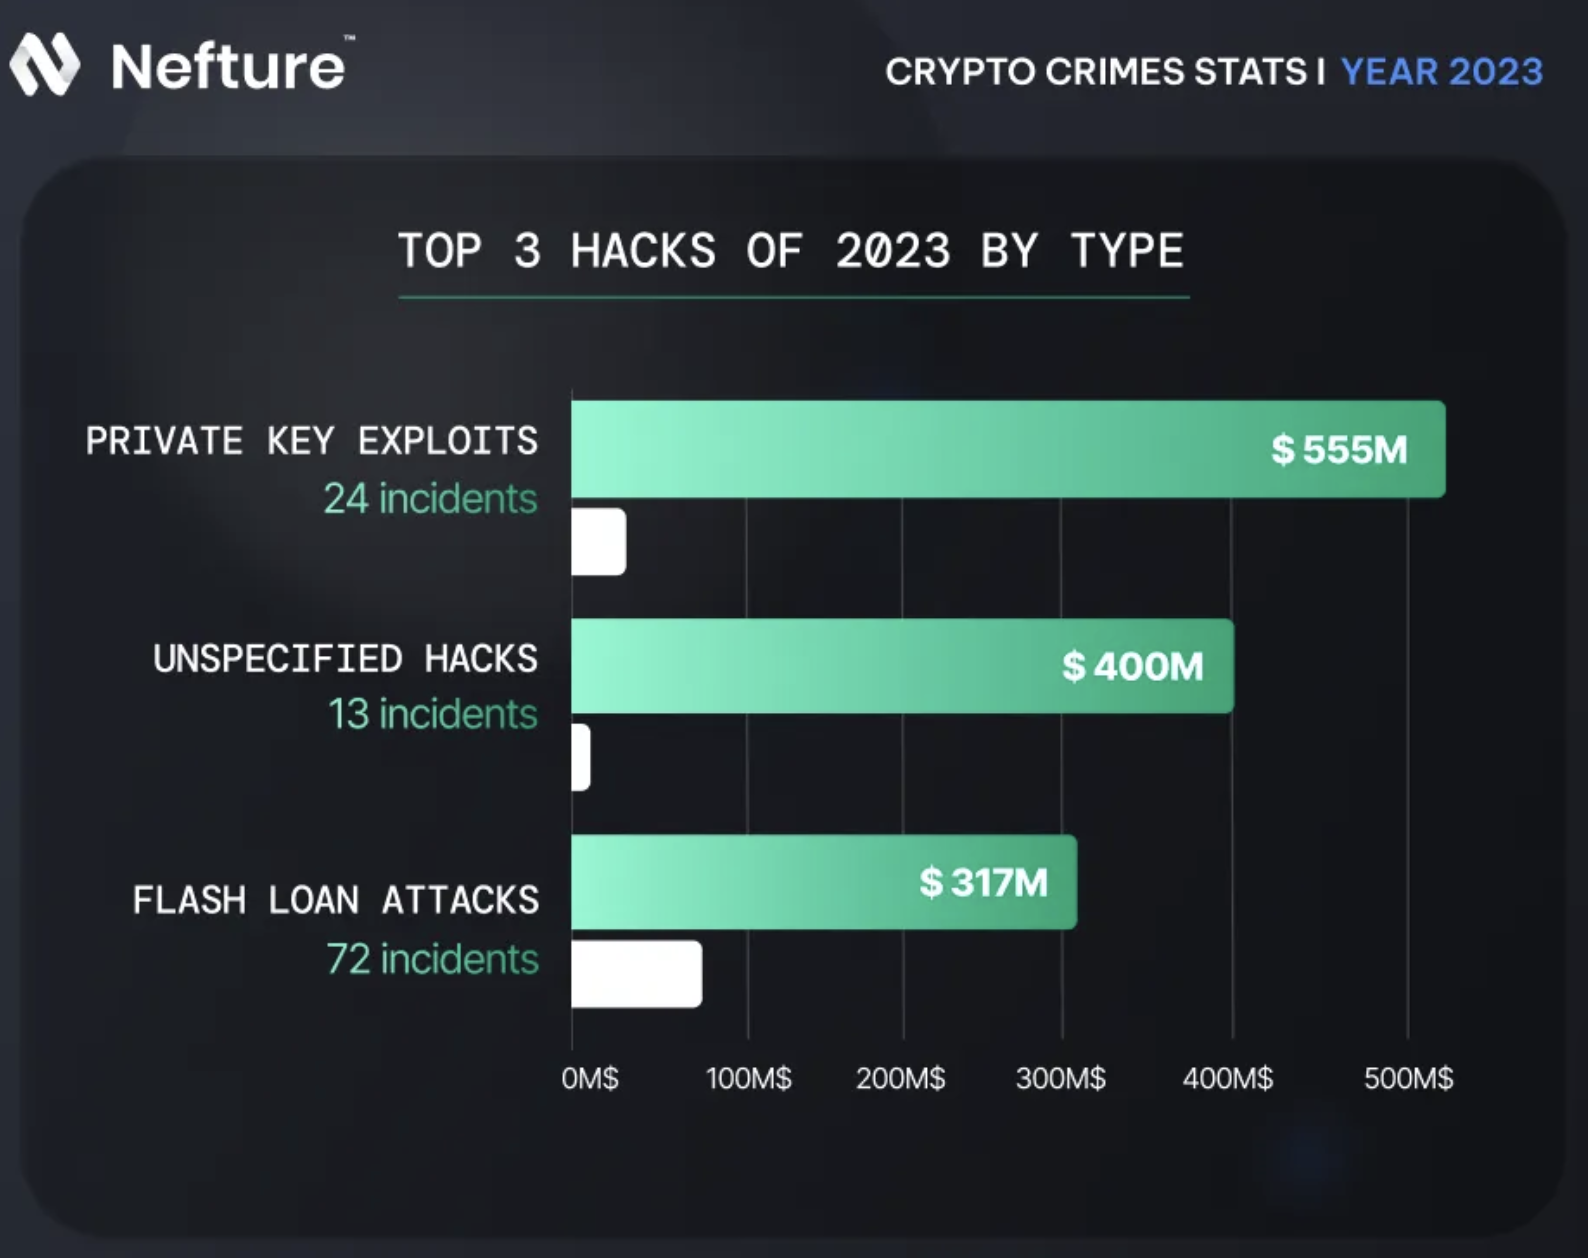
\includegraphics[scale=0.45]{./figures/stolen-pk.png}
	\caption{Total stolen funds value}
\end{figure}

\par A notable aspect that needs to be mentioned is that according to Nefture "Only 16.6\% of the contracts analyzed were managed by multisig wallets"\cite{Nefture2023Hack}. Using a multisig wallet can drastically reduce the probabilty of getting hacked especially if it was set up with multiple ownsers. This method lowers the possibility of unauthorized access to the system by requiring the consent of many parties prior to transactions being completed, adding an extra layer of security.


\section{Purpose}
\label{sec:ch1sec2}

\par The aim of this thesis is to develop a multisig wallet called "Vault" compatible with any EVM (Ethereum Virtual Machine) chain. Vault will provide a secure and efficient solution for managing digital assets across a wide range of blockchain platforms.
\par Vault will be a unified platform for managing digital assets across multiple EVM blockchains such as Ethereum, Base, Polygon etc. Users will be able to store, transfer and receive cryptocurrencies and NFTs easily and securely using a single interface. 
\par Vault is a simple to use multisig wallet that offers increased flexibility and security for managing digital assets. Unlike traditional wallets, Vault does not rely on a single private key, but uses a smart contract to distribute responsibility between multiple people or devices. This approach allows for personalized wallet configuration, perfectly adapting to individual needs and providing granular control over access to funds. Using smart contracts for this also allows for infinite configuration in the future. For features like: Key Recovery, Accounts Whitelisting (trusted accounts the wallet is allowed to interact with), Spending Limits, Subscriptions etc. 
\par Like any other multisig wallet the number of owners, and the approval threshold (the minimum number of signatures (approvals) execute a transaction) can be specified. This enables Vault to be used in a lot of different use cases:
\begin{itemize}
\item Shared Accounts: To enable cooperative fund management, several owners can be set up with a low approval requirement (for example, 1 of 2).
\item Enhanced Security: In order to guarantee access to funds even in the event of a lost private key, users can designate multiple private keys as owners. To improve security, a higher acceptance threshold (such as two out of three) might be specified.
\item Corporate Governance: The company's money can be transparently and democratically controlled by a board of directors acting as wallet owners, with a majority (i.e., 50\% + 1) vote required to approve transactions.
\end{itemize}

\section{Related work}
\label{sec:ch1sec3}

\par Multi-sig wallets offer a more secure solution for managing digital assets by sharing control between multiple people or devices. This section reviews relevant work related to multisig wallets, blockchain security protocols and multi-channel interoperability, contextualizing Vault in the existing landscape.
\par Currenlty some of the most used multisig wallets are:
\begin{itemize}
	\item Gnosis Safe: Since its 2018 launch, users have come to trust it because of its strong security and adaptable features. DApp integration: Allows for use in a variety of DeFi, NFT, and DAO scenarios by integrating with different DApp platforms. Smart contracts that have been audited: The wallet's smart contract code has been examined by recognized professionals, which lowers the possibility of security flaws. Decentralized governance: SafeDAO oversees the wallet's development, guaranteeing openness and participation from the community.
	\item Rabby Wallet: "Rabby Wallet is a Web3 wallet that offers a smooth multi-chain experience by automatically switching to the corresponding chain based on your visited Web3 dApp. Our security rule engine lets you check errors and risks before signing transactions. Rabby Wallet shows you the estimated balance change while you sign a transaction."\cite{rabbywallet}
	\item Argent X Wallet: "Argent is the first non-custodial wallet with no seed phrase and no complexity. With your Argent Vault, enjoy peace of mind through locking and unlocking your account, auto blocking transactions, and setting trusted contacts:"\cite{argent}
\end{itemize}

\par When compared to the other wallets, Vault's interface is far more straightforward and user-friendly. However, the Atlas 2FA feature is the best feature that no one else has. To put it simply, Vault allows you to set up a two-factor authentication code with Google authenticator. This code is required in addition to standard multisig security in order for the transaction to be completed. The best part is that you can configure your multisig to function as a wallet with one owner and one approval signature, but you can also turn on the Atlas for an additional security layer.